\part{ФОРМИРОВАНИЕ ЦЕЛЕВОЙ ФУНКЦИИ}
    \begin{center}
        Целевая функция: $CF=\sum(Y_{\text{э}} - Y_{\text{м}})^2$
    \end{center}

    Неизвестными являются параметры $k$, $b_1$, для оптимизации целевой функции к ней применяется ранее написанный алгоритм. На каждой итерации параметры для расчета нового $y_M$ будут изменяться. Значения остальных переменных остаются такими же, как при вычислении теоретических значений.

    Оптимизация будет выполняться для трех экспериментальных функций $y_{\text{Э1}}, y_{\text{Э2}}, y_{\text{Э3}}$. В результате получаем три пары значений неизвестных параметров.

    \begin{center}
        \begin{tabular}{c|c|c|}
        \cline{2-3}
                                    & k    & $b_1$ \\ \hline
        \multicolumn{1}{|c|}{$CF1$} & 4.16 & 0.938 \\ \hline
        \multicolumn{1}{|c|}{$CF2$} & 4.13 & 0.8   \\ \hline
        \multicolumn{1}{|c|}{$CF3$} & 3.8  & 1.134 \\ \hline
        \multicolumn{1}{|c|}{$y_{\text{сред}}$}   & 4.03  & 0.96   \\ \hline
        \end{tabular}
    \end{center}

    Наложим графики.

    \begin{center}
        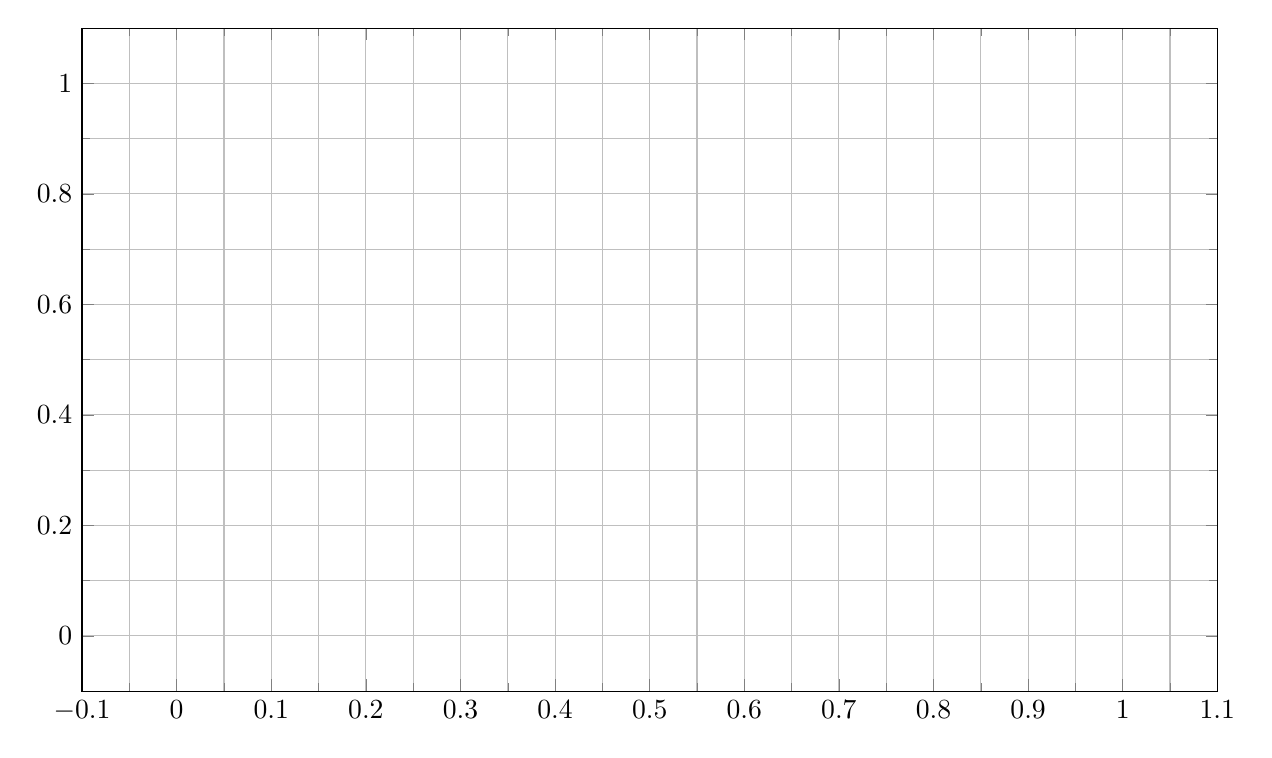
\begin{tikzpicture}
            \begin{axis}[
                width=16cm,
                height=10cm,
                samples=1,
                minor tick num = 1,
                grid = both,
                legend style={at={(0.5,-0.1)},anchor=north}
            ]

            % \addplot[gr1] table {data/1points.dat};
            \addlegendentry{$Y_\text{Т}$}
            % \addplot[gr2] table {data/approx.dat};
            \addlegendentry{$Y_\text{сред}$}

            \end{axis}
        \end{tikzpicture}
    \end{center}

    Так как график, построенный по теоретическим данным практически совпадает с полученным графиком функции с модельными значениями, можно сделать вывод, что оптимизация выполнена верно.
